\chapter{NASM Language}
\section{Structure of a NASM Program}
Like most assemblers, each NASM source line contains some combination of the four fields:
\mint{bash}| label: instruction operands ; comment |
As usual, most of these fields are optional; the presence or absence of any combination of a label, an instruction and a comment is allowed. Of course, the operand field is either required or forbidden by the presence and nature of the instruction field. The structure of a NASM program is presented in the figure \ref{fig:structure}. Generally, you put code in a section called .text and your constant data in a section called .data.
\begin{figure}[ht]
	\centering
	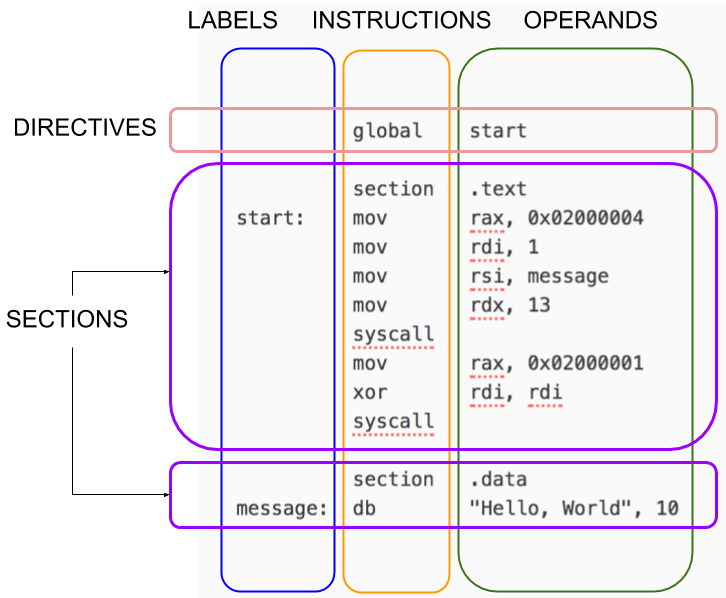
\includegraphics[width=0.8\textwidth]{fig/nasmstructure.png} 
	\caption{Structure of a NASM program. \textit{Tomado de \cite{website:NASM-Tutorial}}}
	\label{fig:structure}
\end{figure}

\section{How to write and read from console?}
In some way we already saw how to write to console in the hello example from chapter 1 (Source Code \ref{listing:hello}). In the section we are going to be more specific.

Writing standalone programs with just system calls is cool, but rare. We would like to use the good stuff in the C library. Remember how in C execution “starts” at the function main? That's because the C library actually has the \textunderscore start label inside itself! The code at \textunderscore start does some initialization, then it calls main, then it does some clean up, then it issues the system call for exit. So you just have to implement main. We can do that in assembly!

In macOS land, C functions (or any function that is exported from one module to another, really) must be prefixed with underscores. The call stack must be aligned on a 16-byte boundary. And when accessing named variables, a rel prefix is required.

As we can see from the program writeRead.asm (Source Code \ref{listing:writeRead}), we have three sections called .data, .bss and .text. We are going to explain the function of each of those.

\subsection{Pseudo-Instructions}
Pseudo-instructions are things which, though not real x86 machine instructions, are used in the instruction field anyway because that’s the most convenient place to put them. The current pseudoinstructions are DB, DW, DD, DQ, DT, DO, DY and DZ; their uninitialized counterparts RESB, RESW, RESD, RESQ, REST, RESO, RESY and RESZ; the INCBIN command, the EQU command, and the TIMES prefix.

\begin{listing}[H]
\inputminted{nasm}{code/writeRead.asm}
\caption{Input and output. writeRead.asm}
\label{listing:writeRead}
\end{listing}

\subsubsection{section .data, initialized varables}
The data section is used for declaring initialized data or constants. This data does not change at runtime. You can declare various constant values, file names, or buffer size, etc. The variables are defined using this directives
\begin{itemize}
\item \texttt{db:} Byte type variable, 8 bits.
\item \texttt{dw:} Word type variable, 16 bits.
\item \texttt{dd:} Double word type variable, 32 bits.
\item \texttt{dq:} Quadruple word type variable, 64 bits.
\end{itemize}
In the given example (Source Code \ref{listing:writeRead}) the variables declared are:
\begin{minted}{nasm}
n_in: db 'What is your first name? ',0 ;For name input
n_out: db 'Your name is %s', 10, 0 ; For name output, 10 is for breakline
f_str: db "%s",0 ;To store the name
\end{minted}

\subsubsection{section .bss, uninitialized variables}
The bss section is used for declaring uninitialized variables. The variables  are defined using thes corresponding directives
\begin{itemize}
\item \texttt{resb:} Reserve space in Bytes units, 1 byte
\item \texttt{resw:} Reserve space in Word units, 2 bytes
\item \texttt{resd:} Reserve space in Double Word units, 4 bytes
\item \texttt{resq:} Reserve space in Quadruple Word units, 8 bytes
\end{itemize}
In the given example (Source Code \ref{listing:writeRead}) the variables are:
\begin{minted}{nasm}
NAME: resq 1 ; to save the name
\end{minted}
Notice how in this example we used \texttt{resq} since we only need the pointer to the start of the string. There are other ways to defined initialized and uninitialized data, you can have a look at the NASM docs to further explanation \cite{website:NASM}.

\subsubsection{section .text, instructions of the program}
Finally in this section we present the instructions for the actual program. In C programming would be something like this:
\begin{minted}[fontsize=\footnotesize]{c}
int main() {
	printf("What is your name? ");
	scanf("%s", &NAME);
	printf("Your name is %s", NAME);
	return 0;
}
\end{minted}

\subsubsection{Definition of other elements}
Other element commonly present are:
\begin{itemize}
\item \textbf{extern} \\
Declare a symbol like external. We use it if we want to access a symbol that is not defined in the file we are assembling, but in another source code file, in which it will have to be defined and declared with the global directive. For example when we use it to invoke the \textit{printf} and \textit{scanf} functions from the C library.

\item \textbf{global}\\
It is the complementary directive of extern. It makes visible a symbol defined in a source code file in other source code files; In this way, we can refer to this symbol in other files using the extern directive.

For example a subroutine that takes two inputs and add them called sum.asm with a global symbol \textunderscore sum can be called from other C program. In our example we have:
\begin{minted}{nasm}
global	 _main
extern	 _printf
extern	 _scanf
\end{minted}
\end{itemize}

\section{Instructions and Addressing Modes}
An assembly instruction consists of an operation code (the name of the instruction) that determines what the instruction should do, plus a set of operands that directly express a data, a record or a memory address; the different ways of expressing an operand in an instruction and the associated procedure that allows obtaining the data is called addressing mode \cite{book:EstComp}. 
\begin{enumerate}
\item \textbf{Instructions without any explicit operand:} opcode \\
\begin{minted}{nasm}
ret	; return from a subroutine
\end{minted}

\item \textbf{Instructions with one operand:} opcode destiny\\
\begin{minted}{nasm}
push rax 	   ; save rax on stack
pop rax         ; load the top of stack on rax
call _printf    ; calls for printf subrutine
inc rax         ; rax=rax+1
\end{minted}

\item \textbf{Instructions with two operands:} opcode destiny, source\\
\begin{minted}{nasm}
mov rbp, rsp  ; move the stack to bas pointer
add rax, 4      ; rax=rax+4
\end{minted}
\end{enumerate}

\subsection{Addressing Modes}
When an operand is in memory, it is necessary to consider which mode of addressing we use to express an operand in an instruction to define the way to access a specific data. Next, we will look at the addressing modes that we can use in an assembly program:

\begin{enumerate}
\item \textbf{Immediate.} In this case, the operand refers to a data found in the instruction itself. There is no need to do any extra memory access to obtain it. We can only use an immediate address as a source operand. For example:

\begin{minted}{nasm}
mov rax, 1				; Immediate mode, loads 1 to rax
\end{minted}

In the example showed, rax needed to be 1 because we have one parameter 

\mint[fontsize=\footnotesize]{c}| printf("Your name is %s", name); |

\item \textbf{Register Direct.} In this case, the operand refers to a data that is stored in a record. In this addressing mode we can specify any general purpose record (data records, index registers and pointer records).

\begin{minted}{nasm}
mov rbp, rsp		; Register direct mode, aligning the stack
\end{minted}

\item \textbf{Memory Direct.} In this case, the operand refers to a data that is stored in a memory location. The operand must specify the name of a memory variable in brackets []; It should be remembered that in NASM syntax the name of a variable without curls is interpreted as the address of the variable and not as the content of the variable. For mac users the next line must be used.

\mint{nasm}| default rel |

In the writeRead.asm (\ref{listing:writeRead}) example we have:

\begin{minted}{nasm}
lea rsi, [NAME]	; Memory direct mode from var [name] to rsi
\end{minted}

where \texttt{lea} means load effective address.

\item \textbf{Stack Mode.} Implicitly works with the top of the stack, by means of the register stack pointer; in the x86-64 architecture this record is called rsp. In the stack we can only store 16-bit and 64-bit values.

There are only two specific instructions designed to work with the stack: \texttt{push} and \texttt{pop}.

\begin{minted}{nasm}
push rbp		; loads base pointer to the stack
pop rbp		; extract base pointer from the stack
\end{minted}
\end{enumerate}

\subsection{Types of instructions}
We can organize the instructions according to the following types:
\begin{enumerate}
\item \textbf{Data Transfer Instructions.}
	\begin{itemize}
	\item \texttt{mov dest, src}: generic instruction to move a data from a source to a destination.
	\item \texttt{push src}: instruction that moves the operand of the instruction to the top of the stack.
	\item \texttt{pop dest}: moves the data that is on top of the stack to the operand destination.
	\end{itemize}

\item \textbf{Arithmetic and Comparison Instructions.}
	\begin{itemize}
	\item \texttt{add dest, src}: arithmetic sum of the two operands.
	\item \texttt{sub dest, src}: arithmetic subtract of the two operands.
	\item \texttt{inc dest}: increments the operand in one unit.
	\item \texttt{dec dest}: decrements the operand in one unit.
	\item \texttt{mul src}: integer multiplication without sign.
	\item \texttt{imul src}: integer multiplication with sign.
	\item \texttt{div src}: integer division without sign.
	\item \texttt{idiv src}: integer division with sign.
	\item \texttt{neg dest}: arithmetic negation, 2 complement's.
	\item \texttt{cmp dest, src}: comparison between two operands, it subtracts them without saving the result.
	\end{itemize}

\item \textbf{Logic Instructions.}
	\begin{itemize}
	\item \texttt{and dest, src}: logic operation 'and'.
	\item \texttt{or dest, src}: logic operation 'or'.
	\item \texttt{xor dest, src}: logic operation 'exclusive or'.
	\item \texttt{not dest, src}: logic negation bit by bit.
	\end{itemize}
	
\item \textbf{Sequence Instructions.}\\
\textit{Unconditional jump}
	\begin{itemize}
	\item \texttt{jmp label}: Unconditional jump to label.
	\end{itemize}
	
\textit{Jumps that query a concrete result bit}
	\begin{itemize}
	\item \texttt{je label / jz label}: jumps if equal, jumps if bit zero is active.
	\item \texttt{jne label / jnz label}: jumps if not equal, jumps if bit zero is not active.
	\end{itemize}	

\textit{Conditional jump without considering the sign}
	\begin{itemize}
	\item \texttt{jb label}: jumps if below.
	\item \texttt{jbe label}: jumps if below or equal.
	\item \texttt{ja label}: jumps if above.
	\item \texttt{jae label}: jumps if above or equal.
	\end{itemize}	

\textit{Conditional jump considering the sign}
	\begin{itemize}
	\item \texttt{jl label}: jumps if lesser.
	\item \texttt{jle label}: jumps if lesser or equal.
	\item \texttt{jg label}: jumps if greater.
	\item \texttt{jge label}: jumps if greater or equal.
	\end{itemize}	

\textit{Other sequence instructions}
	\begin{itemize}
	\item \texttt{loop label}: decrements rcx and jumps if rcx is not zero.
	\item \texttt{call label}: call to a subroutine.
	\item \texttt{ret}: returns from a subroutine.
	\end{itemize}	
\end{enumerate}
